\documentclass[]{article}
\usepackage{lmodern}
\usepackage{amssymb,amsmath}
\usepackage{ifxetex,ifluatex}
\usepackage{fixltx2e} % provides \textsubscript
\ifnum 0\ifxetex 1\fi\ifluatex 1\fi=0 % if pdftex
  \usepackage[T1]{fontenc}
  \usepackage[utf8]{inputenc}
\else % if luatex or xelatex
  \ifxetex
    \usepackage{mathspec}
  \else
    \usepackage{fontspec}
  \fi
  \defaultfontfeatures{Ligatures=TeX,Scale=MatchLowercase}
\fi
% use upquote if available, for straight quotes in verbatim environments
\IfFileExists{upquote.sty}{\usepackage{upquote}}{}
% use microtype if available
\IfFileExists{microtype.sty}{%
\usepackage{microtype}
\UseMicrotypeSet[protrusion]{basicmath} % disable protrusion for tt fonts
}{}
\usepackage[margin=1in]{geometry}
\usepackage{hyperref}
\hypersetup{unicode=true,
            pdftitle={Spatial Analysis of Crime Patterns in London},
            pdfauthor={Ng Jia Wen \& Junju Ng},
            pdfborder={0 0 0},
            breaklinks=true}
\urlstyle{same}  % don't use monospace font for urls
\usepackage{longtable,booktabs}
\usepackage{graphicx,grffile}
\makeatletter
\def\maxwidth{\ifdim\Gin@nat@width>\linewidth\linewidth\else\Gin@nat@width\fi}
\def\maxheight{\ifdim\Gin@nat@height>\textheight\textheight\else\Gin@nat@height\fi}
\makeatother
% Scale images if necessary, so that they will not overflow the page
% margins by default, and it is still possible to overwrite the defaults
% using explicit options in \includegraphics[width, height, ...]{}
\setkeys{Gin}{width=\maxwidth,height=\maxheight,keepaspectratio}
\IfFileExists{parskip.sty}{%
\usepackage{parskip}
}{% else
\setlength{\parindent}{0pt}
\setlength{\parskip}{6pt plus 2pt minus 1pt}
}
\setlength{\emergencystretch}{3em}  % prevent overfull lines
\providecommand{\tightlist}{%
  \setlength{\itemsep}{0pt}\setlength{\parskip}{0pt}}
\setcounter{secnumdepth}{5}
% Redefines (sub)paragraphs to behave more like sections
\ifx\paragraph\undefined\else
\let\oldparagraph\paragraph
\renewcommand{\paragraph}[1]{\oldparagraph{#1}\mbox{}}
\fi
\ifx\subparagraph\undefined\else
\let\oldsubparagraph\subparagraph
\renewcommand{\subparagraph}[1]{\oldsubparagraph{#1}\mbox{}}
\fi

%%% Use protect on footnotes to avoid problems with footnotes in titles
\let\rmarkdownfootnote\footnote%
\def\footnote{\protect\rmarkdownfootnote}

%%% Change title format to be more compact
\usepackage{titling}

% Create subtitle command for use in maketitle
\newcommand{\subtitle}[1]{
  \posttitle{
    \begin{center}\large#1\end{center}
    }
}

\setlength{\droptitle}{-2em}

  \title{Spatial Analysis of Crime Patterns in London}
    \pretitle{\vspace{\droptitle}\centering\huge}
  \posttitle{\par}
    \author{Ng Jia Wen \& Junju Ng}
    \preauthor{\centering\large\emph}
  \postauthor{\par}
      \predate{\centering\large\emph}
  \postdate{\par}
    \date{28/10/2018}


\usepackage{amsthm}
\newtheorem{theorem}{Theorem}[section]
\newtheorem{lemma}{Lemma}[section]
\theoremstyle{definition}
\newtheorem{definition}{Definition}[section]
\newtheorem{corollary}{Corollary}[section]
\newtheorem{proposition}{Proposition}[section]
\theoremstyle{definition}
\newtheorem{example}{Example}[section]
\theoremstyle{definition}
\newtheorem{exercise}{Exercise}[section]
\theoremstyle{remark}
\newtheorem*{remark}{Remark}
\newtheorem*{solution}{Solution}
\begin{document}
\maketitle

{
\setcounter{tocdepth}{2}
\tableofcontents
}
\pagebreak

\pagebreak

\section{Introduction}\label{introduction}

Crime (and its prevention and responses) is associated with significant
social and economic costs. In England and Wales, the total cost of
crimes against individuals and businesses is ?50.1 billion and ?8.7
billion respectively in 2015/16 alone (Brand and Price
\protect\hyperlink{ref-Brand2014}{2014}). A significant portion of these
costs are incurred in London, given that about 20\% of crimes in England
and Wales occurs in London (Mayor of London
\protect\hyperlink{ref-MayorofLondon2016}{2016}).

Consequently, much work has been done to understand the occurrence of
crime, and to predict crime. To date, the spatial concentration of crime
in cities is well-established in the literature (Malleson and Andresen
\protect\hyperlink{ref-Malleson2016}{2016}). (Sherman, Gartin, and
Buerger \protect\hyperlink{ref-Sherman1989}{1989})'s seminal analysis of
predatory crime in Minneapolis revealed that 50\% of police calls come
from 3\% of street segments, indicating that crime hotspots, down to the
street level, are present within cities. Recent works have thus focussed
on trying to improve spatial analysis techniques for crime.
Specifically, (Chainey, Tompson, and Uhlig
\protect\hyperlink{ref-Chainey2008}{2008}) examined the use of different
hotspot mapping techniques to predict spatial patterns of crime in
Camden and Islington local authority district areas in London. Other
workers have been working on developing techniques to examine
spatial-temporal patterns of crime (Cheng and Williams
\protect\hyperlink{ref-Cheng2012}{2012}), in order to understand how
crime develops and evolves to improve crime prediction.

Given that a significant portion of crimes in England and Wales occurs
in London and the occurrence of crime is non-random, this study will
therefore examine spatial crime patterns in London. Specifically, this
study aims to answer two main questions: 1) where do crime types occur?
2) what factors are associated with the occurrence of different types of
crime?

\textbf{Study area}

London is a thriving metropolis in the United Kingdom with a population
of 8.8 million. Beyond the large residential population, London also
attracts a huge number of visitors, with more than 56 million overnight
stays from tourists in 2016 (Mayor of London
\protect\hyperlink{ref-MayorofLondon2016}{2016}).

London consists of 33 local government districts (32 London Boroughs and
the City of London). The City of London Police is the police force
responsible for law enforcement within the City of London while the
Metropolitan Police Service is reponsible for policing the Greater
London region, excluding the City of London. Greater London can be split
into 4835 geographic regions known as lower layer super output
areas(LSOAs) for the purposes of reporting small-area statistics. These
LSOAs will form the basis of the analysis.

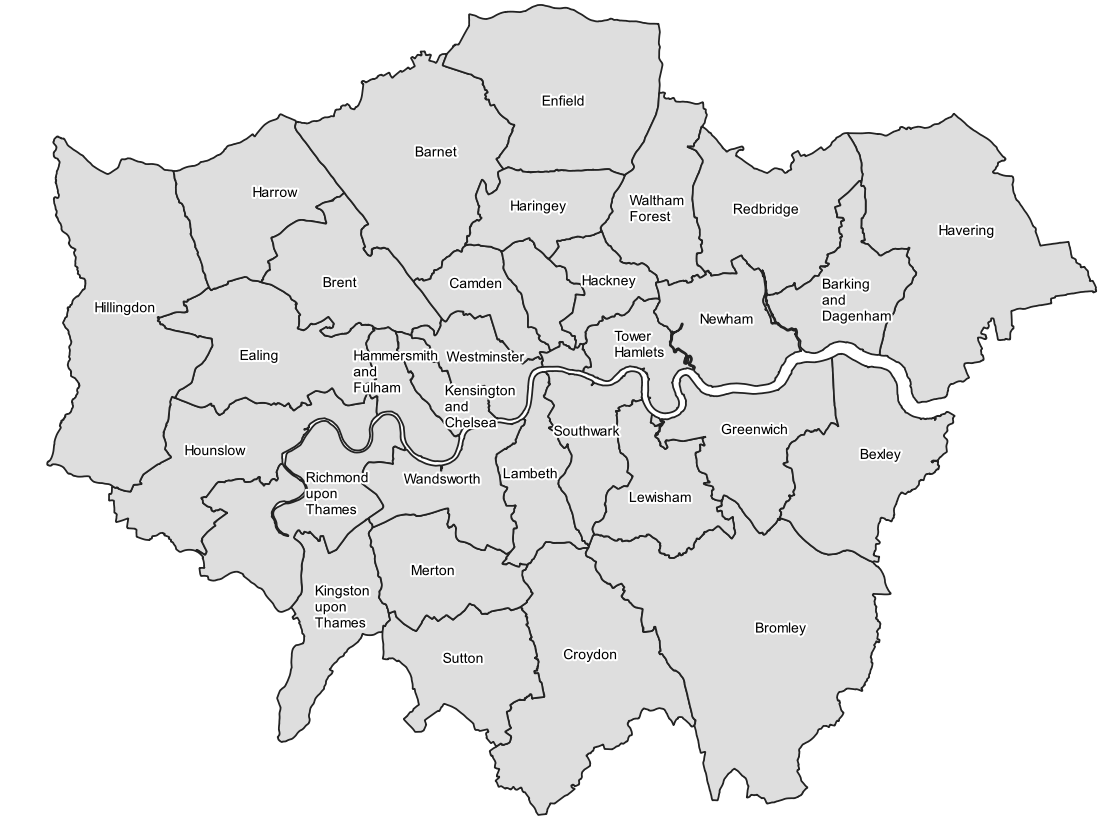
\includegraphics[width=2.60417in]{pictures/London.png} \pagebreak

\section{Data description}\label{data-description}

Official geocoded crime data from London is required to analyse spatial
patterns of crime. Crime data in London for a one-year period (1 January
2017 to 31 December 2017) from the Metropolitan Police and the City of
London Police was used. These data are taken from the Metropolitan
Police and the City of London Police because they are the two police
forces covering the London and Greater London area. The data was
obtained via the police.uk website as a CSV file. Whilst most crimes are
geocoded, some reported crimes do not have a location and are therefore
excluded from the analysis. The effect on excluding crimes without
locations from the analysis is anticipated to be minimal, as they only
form a small proportion of reported crimes (5.3\% for the City of London
Police, and 1.2\% for the Metropolitan Police).

The geocoded crime data are categorised into 14 crime types: anti-social
behaviour, bicycle theft, burglary, criminal damage and arson, drugs,
other crime, other theft, possession of weapons, public order, robbery,
shoplifting, theft from a person, vehicle crime, and violence and sexual
offences. Geomasking techniques are applied to the data to reduce their
spatial accuracy for privacy purposes. Specifically, each crime is
mapped to its nearest map point on the master list of map points kept by
the Home Office (Home Office \protect\hyperlink{ref-Office2019}{2019}).
However, analysis by (Tompson et al.
\protect\hyperlink{ref-Tompson2015}{2015}) reveals that at the lower
super output area (LSOA) level, 85\% of areas exhibited no statistically
significant difference between the masked and raw crime data. Hence,
analysis of patterns in crime will predominantly be conducted at the
LSOA level in this study.

2011 census data at the LSOA level was also downloaded from the London
Datastore. This is to obtain information about the total resident
population in each London LSOA to calculate crime rates in each LSOA.

In addition, industrial landuse areas are obtained from OpenStreetMap
using the overpass API as a polygon dataset. This is to observe if
trends between the occurrence of crimes and industrial areas exist. A
point dataset of the location of entertainment outlets (defined as pubs,
bars, and restaurants) in London is also obtained from OpenStreetMap.
The information from OpenStreetMap is crowd-sourced, and not created by
geospatial experts. Thus, some inaccuracies may be present in the
dataset (Basiri et al. \protect\hyperlink{ref-Basiri2016}{2016}).
However, corroboration of the industrial landuse polygons with aerial
imagery and street imagery from Google Maps shows that the data is
generally accurate, and therefore suitable for broader-scale exploratory
analysis. Further verification of the location of entertainment outlets
also suggests that the dataset is broadly up-to-date.

\pagebreak

\section{Exploratory Spatial Data
Analysis}\label{exploratory-spatial-data-analysis}

An exploratory analysis of the crime data will be conducted in this
section.

A total of 1,048,712 crimes were reported in 2017. Of these crimes,
1,035,826 (98.7\%) have a location. As discussed previously, only the
geocoded crimes will be used in the analysis.

\textbf{Variations in Crime by Type}

The barplot below depicts the frequency of crimes by crime type in
London in 2017 (Figure \ref{fig:barplot}). Over 40\% of reported crimes
in London come from 2 categories - anti-social behaviour (22.0\%) and
violence and sexual offences (20.7\%). The next two most significant
crime types making up 20\% of crimes are other theft (10.5\%) and
vehicle crime (10.0\%). 36.9\% of crimes fall under the remaining 10
crime types. As such, different types of crimes are reported at
different frequencies, with antisocial behaviour and violence and sexual
offences being the most commonly reported crimes, followed by vehicle
crime and other theft.

\begin{figure}
\centering
\includegraphics{geo_project_r_files/figure-latex/barplot-1.pdf}
\caption{\label{fig:barplot}2017 London crime counts by crime type}
\end{figure}

\textbf{Variations in Crime by Type and Month}

A line graph of crime count by type and month (Figure
\ref{fig:linegraph}) is plotted to examine temporal patterns in crime in
London across the year. Figure \ref{fig:linegraphnoASBVSO} depicts a
similar graph, without anti-social behaviour and violence and sexual
offences, in order to better observe trends in the other crime types.

From Figure \ref{fig:linegraph}, it is evident that the frequency of
some crime types varies throughout the year. For instance, reports of
anti-social behaviour appear to peak in July and August. Burglary
reports appear to increase between October and January, while bicycle
theft reports appear to increase between May and October (Figure
\ref{fig:linegraphnoASBVSO}).

\begin{figure}
\centering
\includegraphics{geo_project_r_files/figure-latex/linegraph-1.pdf}
\caption{\label{fig:linegraph}2017 London crime count by type and month}
\end{figure}

\begin{figure}
\centering
\includegraphics{geo_project_r_files/figure-latex/linegraphnoASBVSO-1.pdf}
\caption{\label{fig:linegraphnoASBVSO}2017 London crime count by type and
month (excluding anti-social behaviour and violence and sexual offences}
\end{figure}

\textbf{Variations in Crime by LSOA}

Crime counts are also examined by LSOA, in order to study the
distribution of crime in London. From Table \ref{tab:LSOAstats}, it is
evident that crime counts vary significantly between LSOAs. Few LSOAs
have extremely high crime counts, while 50\% of LSOAs have crime counts
between 64 and 211. Consequently, the jenks classification scheme will
be used to map the distribution of crime counts across London, to
minimise the variation within each class but highlight differences
between classes.

\begin{table}

\caption{\label{tab:LSOAstats}Crime Count Statistics by LSOA}
\centering
\begin{tabular}[t]{l|r}
\hline
  & Value\\
\hline
Minimum & 1.0\\
\hline
1st Quartile & 64.0\\
\hline
Median & 127.0\\
\hline
Mean & 175.3\\
\hline
3rd Quartile & 211.0\\
\hline
Maximum & 7329.0\\
\hline
\end{tabular}
\end{table}

Crime count maps are plotted to visualise the spatial distribution of
crime across London. The crime count map (Figure
\ref{fig:crimecountmap}) illustrates the total number of reported crimes
in each LSOA in 2017. This depicts regions with the highest number of
crimes. By visual inspection, crime counts are highest in central
London, although some regions with higher crime counts are present along
the river Thames in East London, the Lea Valley and in Hillingdon.
However, crime counts do not consider that LSOAs have unequal areas and
do not accurately represent crime density.

\includegraphics{geo_project_r_files/figure-latex/crimecountmap-1.pdf}
Thus, a crime rate map (Figure \ref{fig:crimeratemap}), derived by
taking the crime count divided by the resident population in the
corresponding LSOA and then multipled by 1000 (i.e.~crime count per 1000
residents), is plotted. These crime rate maps allow for the assessment
of the risk of crime in each LSOA (P. L. Brantingham and Brantingham
\protect\hyperlink{ref-Brantingham1997}{1997}). However, it is to be
noted that resident populations are used to calculate crime rate. Thus,
regions with a low resident population (but high pedestrian population
e.g.~commercial areas) would have an inflated crime rate.

Visually, although there are some differences between the crime rate and
crime count maps, the regions with the highest crime counts are also the
regions with the highest crime rates. However, a number of regions
outside of central London with slightly higher crime counts (284 to 873)
have lower-than-expected crime rates. This indicates that residential
population does not have a significant influence on crime counts, except
when crime counts are slightly elevated and occur in LSOAs outside
central London (presumably with a higher residential population).

\includegraphics{geo_project_r_files/figure-latex/crimeratemap-1.pdf}
\pagebreak

\section{Methodology}\label{methodology}

Based on our exploratory data analysis, different crime types have
different counts and spatial variations. As such, we have decided to
analyse two different crime types in isolation: Violence and Sexual
Offences (VSO), and Vehicle crime.

VSO is one of the most commonly reported, as well as the more severe
crimes that bring about damage to people and property. Vehicle crime is
chosen due to its unique nature in that it can be committed without
direct contact with the victim, unlike violence and sexual offences
which often requires direct contact with the victim, thus making it an
interesting constrast to study.

As the two crime types have its own spatial pattern and are likely to be
caused by different factors, the methodology that we undertake will be
different for each of them.

\subsection{Methods in Analysing Violence and Sexual
Offences}\label{methods-in-analysing-violence-and-sexual-offences}

A spatial point pattern analysis was done on the City of London 001F
(COL001F) LSOA.

Two hypotheses were made in the process of analysing VSO crime patterns
in the LSOA:

\begin{verbatim}
H1. VSO crimes are randomly distributed in COL001F 

H2. VSO crime locations positively correlate with the locations of entertainment outlets
\end{verbatim}

The reason for these hypotheses will be made clearer in section 5.1.

Here is the methodology employed to investigate the hypotheses:

\begin{enumerate}
\def\labelenumi{\arabic{enumi}.}
\tightlist
\item
  Test H1 with Quadrat Counting

  \begin{itemize}
  \tightlist
  \item
    If homogenous, find out if there is clustering with Ripley's K
    Function.

    \begin{itemize}
    \tightlist
    \item
      If there is clustering, H1 is rejected.
    \item
      If not, H1 is accepted.
    \end{itemize}
  \item
    If non-homogenous, use Kernel Density Estimation to identify areas
    with high intensity.

    \begin{itemize}
    \tightlist
    \item
      H1 is rejected.
    \end{itemize}
  \end{itemize}
\item
  Test H2 with Inhomogenous K cross function

  \begin{itemize}
  \tightlist
  \item
    If Inhomogenous K cross function reveals positive correlation, H2 is
    accepted.
  \item
    If Inhomogenous K cross function reveals no correlation, H2 is
    rejected.
  \item
    If Inhomogenous K cross function reveals negative correlation, H2 is
    rejected.
  \end{itemize}
\end{enumerate}

The following statistical methods were used in the process:

\begin{enumerate}
\def\labelenumi{\arabic{enumi}.}
\item
  Quadrat Counting

  To check for homogeneity is to determine whether regions of equal area
  contain roughly equal number of points.

  \begin{figure}
  \centering
  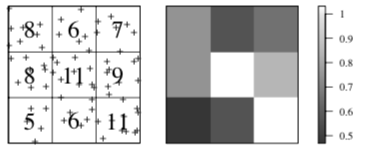
\includegraphics{pictures/quadratcount.png}
  \caption{Picture 1 shows Quadrat counting for Swedish Pines data.
  Left: Quadrat counts. Right intensity. ({\textbf{???}})}
  \end{figure}

  In quadrat counting, the observation window W is divided into
  subregions \(B_{1},...,B_{m}\) called quadrats. The numbers of points
  falling in each quadrat is counted. If the spatial point process is
  homogeneous, the intensity for each quadrat should be equal `on
  average'-- the expected count in each quadrat is proportional to the
  area of the quadrat. Otherwise, the spatial point process is
  inhomogeneous. ({\textbf{???}})
\item
  Chi-sq test

  The Chi-sq test is used to determine whether there is a significance
  difference between the observed number points and the expected number
  of points in each quadrats, where chi-squared can be computed via:

  \(\chi^2=\sum_{i=1}^m\frac{(k_i-\bar{\lambda})^2}{\bar{\lambda}}\)

  If there is a significant difference, then we can reject the null
  hypothesis that the spatial point process is homogeneous as it is not
  behaving in the way it is expected to behave.
\item
  Kernel Density Estimation

  Kernel Density Estimation (KDE) is a method for estimating the
  probability density function of a random variable. It can be used to
  extract the relative likelihood of obtaining a particular value on a
  random drawn. In spatial analysis, KDE can be used to estimate how the
  density of a point process varies across space. ({\textbf{???}})

  A KDE can be written as:
  \(\hat{f}(x,y)=\frac{1}{nh^2}\sum_{i=1}^nk_s(\frac{x-x_i}{h_s}\frac{y-y_i}{h_s})\)

  where \(n\) is the number of points; \(x_{i}\) and \(y_{i}\) are the
  coordinates of the point \(i\), \(i\) = 1,2, \ldots{} , \(n\);
  \(h_{s}\) is the bandwidth of a spatial kernel \(k_{s}\).
\item
  Inhomogenous K cross function

  The inhomogenous K cross function measures whether 2 spatial point
  patterns are correlated, with the assumption that the spatial point
  patterns are inhomogenous.

  \(K_{ij}(r) = \frac{1}{\lambda_{j}}E[t(u,r,X^{j} | u \epsilon X^{i} )]\)

  For any pair of types \(i\) and \(j\), the multitype K-function
  \(K_{ij}(r)\), also called the bivariate or cross-type K-function, is
  the expected number of points of type \(j\) lying within a distance
  \(r\) of a typical point of type \(i\), standardised by dividing by
  the intensity of points of type \(j\), adjusted for spatially varying
  intensity. ({\textbf{???}})
\item
  Monte-Carlo Simulation

  The monte-carlo simulation is used to generate 100 simulations of a
  point pattern according to a specified probability distribution, in
  order to test whether the result from a test is statistically
  significant.
\end{enumerate}

\subsection{Methods in Analysing Vehicle
Crime}\label{methods-in-analysing-vehicle-crime}

Vehicle data was first mapped in terms of crime count and crime count
per 1000 resident population. These choropleth maps were produced using
the jenks classification scheme, to accentuate the variance between
classes, and minimise the variance within each class. Visual inspection
of the maps suggests that vehicle crime rates appear to concentrate in
regions. Thus, the Moran's I was used to test for spatial
autocorrelation.

The Moran's I (Moran \protect\hyperlink{ref-Moran1950}{1950}) is a
weighted correlation coefficient that measures if the spatial data
sampled at adjacent locations are correlated with one another. It
measures a single average spatial autocorrelation across the entire
area. The Moran's I is calculated using the following equation:

\[I=\frac{n} {\sum_{i}\sum_{j}w_{ij}} \frac{\sum_{i}\sum_{j}w_{ij}(x_i-\bar{x})(x_j-\bar{x})} {\sum_{i}(x_i-\bar{x})^2}\]

Where \(n\) is the number of LSOAs, \(w_{ij}\) is the element of a
spatial weight matrix \(W\) giving the spatial weight between LSOAs
\(i\) and \(j\),\\
\(x_i\) and \(x_j\) are the vehicle crime rates measured at LSOAs \(i\)
and \(j\) respectively and \(i,j=1,2,...,n\),\\
\(\bar{x}\) is the mean of \(x\) (i.e.~the mean LSOA vehicle crime rate)

A expectation of I under a null hypothesis is \(\frac{-1} {n-1}\).
Values greater than that indicate a positive spatial autocorrelation,
while values smaller than that indicate a negative spatial
autocorrelation.

A local Moran's I (Anselin \protect\hyperlink{ref-Anselin1995}{1995}),
\(I_i\), was subsequently calculated for each LSOA, to determine the
spatial autocorrelation between a given LSOA and its adjacent LSOAs.
This is to observe if variations in spatial autocorrelation exist. The
local Moran's I can be calculated using the following equation:

\[I_i=\frac{z_i}{m_2}\sum_{j}w_{ij}z_j\]

Where \(z_i = x_i-\bar{x}\), \(z_j = x_j-\bar{x}\),
\(m_2=\frac{1}{n}\sum_{i}z_i^2\), \(\bar{x}\) is the mean vehicle crime
rate, \(x\), at \(n\) LSOAs and \(i=1,2,...,n\)

The expectation of \(I_i\) is \(\frac{-w_i}{(n-1)}\), where
\(-w_i=\sum_{j}w_{ij}\). Local hotspots of positive or negative
autocorrelation will be present if vehicle crime rates are spatially
heterogeneous.

The areas with high vehicle crime rates and which are statistically
significant high-high clusters are then analysed using Google Map
imagery. Further analysis is also conducted with industrial landuse data
from OpenStreetMap. \pagebreak

\section{Results and discussion}\label{results-and-discussion}

Two crime types, violence and sexual offences, and vehicle crime have
been used for further analysis. Examination of violence and sexual
offences will be conducted, as it is one of the most commonly reported,
as well as more severe crimes that bring about damage to people and
property. Vehicle crime refers to any theft, tampering, or interference
with motor vehicles (Home Office
\protect\hyperlink{ref-Office2019}{2019}). It is chosen for further
analysis as it is one of the more commonly reported crimes (excluding
violence and sexual offences). Vehicle crime can also be committed
without direct contact with the victim, unlike violence and sexual
offences which often requires direct contact with the victim.

As the nature of violence and sexual offences, and vehicle crime
differs, examination of the spatial distribution of the two crime types
in London will allow for better understanding of the factors influencing
the occurrence of these two crimes.

\subsection{Analysing Violence and Sexual
Offences}\label{analysing-violence-and-sexual-offences}

By plotting the occurrence of violence and sexual offences per 1000
people on a chloropeth, we get the following map below:

\includegraphics{geo_project_r_files/figure-latex/unnamed-chunk-4-1.pdf}

This map shows us that VSO crimes are mainly concentrated in central
london, with a few LSOAs having mid-range crime density dispersed across
london.

Ranking the LSOAs by crime density, we obtain the following rank table,
showing the top 20 LSOAs with the highest crime rates (crime count per
1000 people):

\begin{table}

\caption{\label{tab:top20}20 LSOAs with the highest crime rates}
\centering
\begin{tabular}[t]{l|r}
\hline
LSOA name & Crime Rate\\
\hline
City of London 001F & 602.4904\\
\hline
Westminster 013E & 594.0426\\
\hline
Westminster 018A & 520.2840\\
\hline
Westminster 018C & 342.8899\\
\hline
Westminster 013B & 304.1843\\
\hline
Camden 021A & 259.9595\\
\hline
Hackney 027G & 254.5341\\
\hline
Lambeth 011B & 244.0074\\
\hline
Kingston upon Thames 009C & 214.7472\\
\hline
Hillingdon 031A & 195.8538\\
\hline
Havering 013C & 193.6538\\
\hline
Islington 004B & 186.2427\\
\hline
Newham 013G & 184.6803\\
\hline
Croydon 027B & 183.4756\\
\hline
Sutton 012D & 183.0226\\
\hline
Greenwich 004E & 173.0580\\
\hline
Westminster 013F & 165.9919\\
\hline
Westminster 018B & 164.5708\\
\hline
Hammersmith and Fulham 004A & 162.2313\\
\hline
Greenwich 036B & 161.7647\\
\hline
\end{tabular}
\end{table}

We select the City of London 001F (COL001F) to do our analysis as it has
the highest crime density. We are also interested to investigate why
this is so.

\subsubsection{Analysing Violence and Sexual Offences in City of London
001F}\label{analysing-violence-and-sexual-offences-in-city-of-london-001f}

\begin{verbatim}
## OGR data source with driver: ESRI Shapefile 
## Source: "C:\Users\Junju\Desktop\Masters\Term 1\Spatial Analysis and Geocomputation\Geocomputation\boundaries\COL001F_roads\COL001F_roads.shp", layer: "COL001F_roads"
## with 4303 features
## It has 8 fields
\end{verbatim}

By plotting the spatial distribution of the crimes on a map (see
@ref(fig:COL001F\_map\_w\_roads)), we can make our first hypothesis:

H1. VSO crimes are randomly distributed in the City of London 001F LSOA

To test for H1, we employ the use of quadrat counting. If the spatial
pattern is homogeneous, each quadrat should have roughly the same amount
of intensity (points per area).\\
\includegraphics{geo_project_r_files/figure-latex/COL001F-homo-1.pdf}

A chi-sq test gives the following results:

\begin{verbatim}
## 
##  Chi-squared test of CSR using quadrat counts
##  Pearson X2 statistic
## 
## data:  COL001F_ppp
## X2 = 253.11, df = 27, p-value < 2.2e-16
## alternative hypothesis: two.sided
## 
## Quadrats: 28 tiles (irregular windows)
\end{verbatim}

As the p-value is less than 0.05, it rejects the null hypothesis that
the crimes are homogeneous.

Next, we use the Kernel Density Estimation to visualise the different
intensities of the VSO crime on the map.\\
\includegraphics{geo_project_r_files/figure-latex/COL001F-KDE-1.pdf}

From the map, clusters of VSO crime seem to occur North-East of City of
London 001F. To understand why this is so, we can study the area in more
detail (red box).

\begin{figure}
\centering
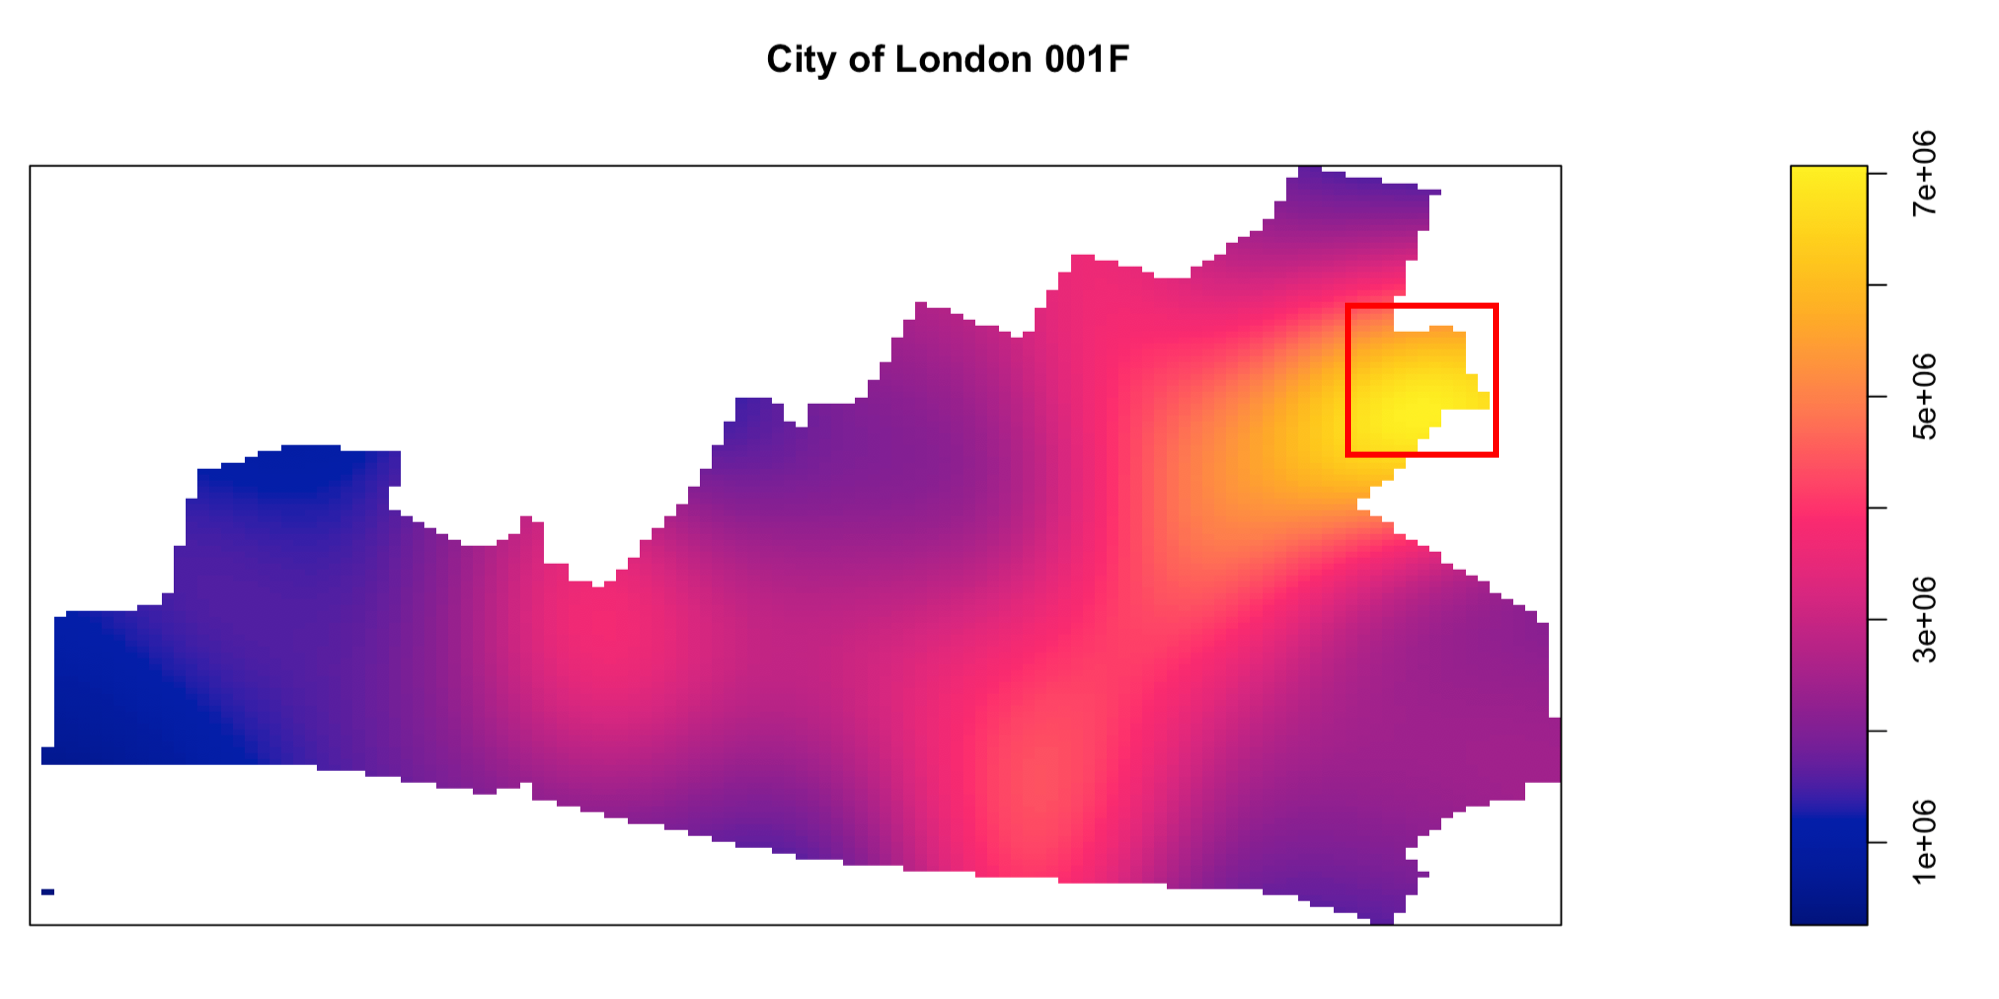
\includegraphics{pictures/COL001F_Hotspot_box.png}
\caption{}
\end{figure}

The street level view reveals a hotspot of 67 VSO crimes in the region.

\begin{figure}
\centering
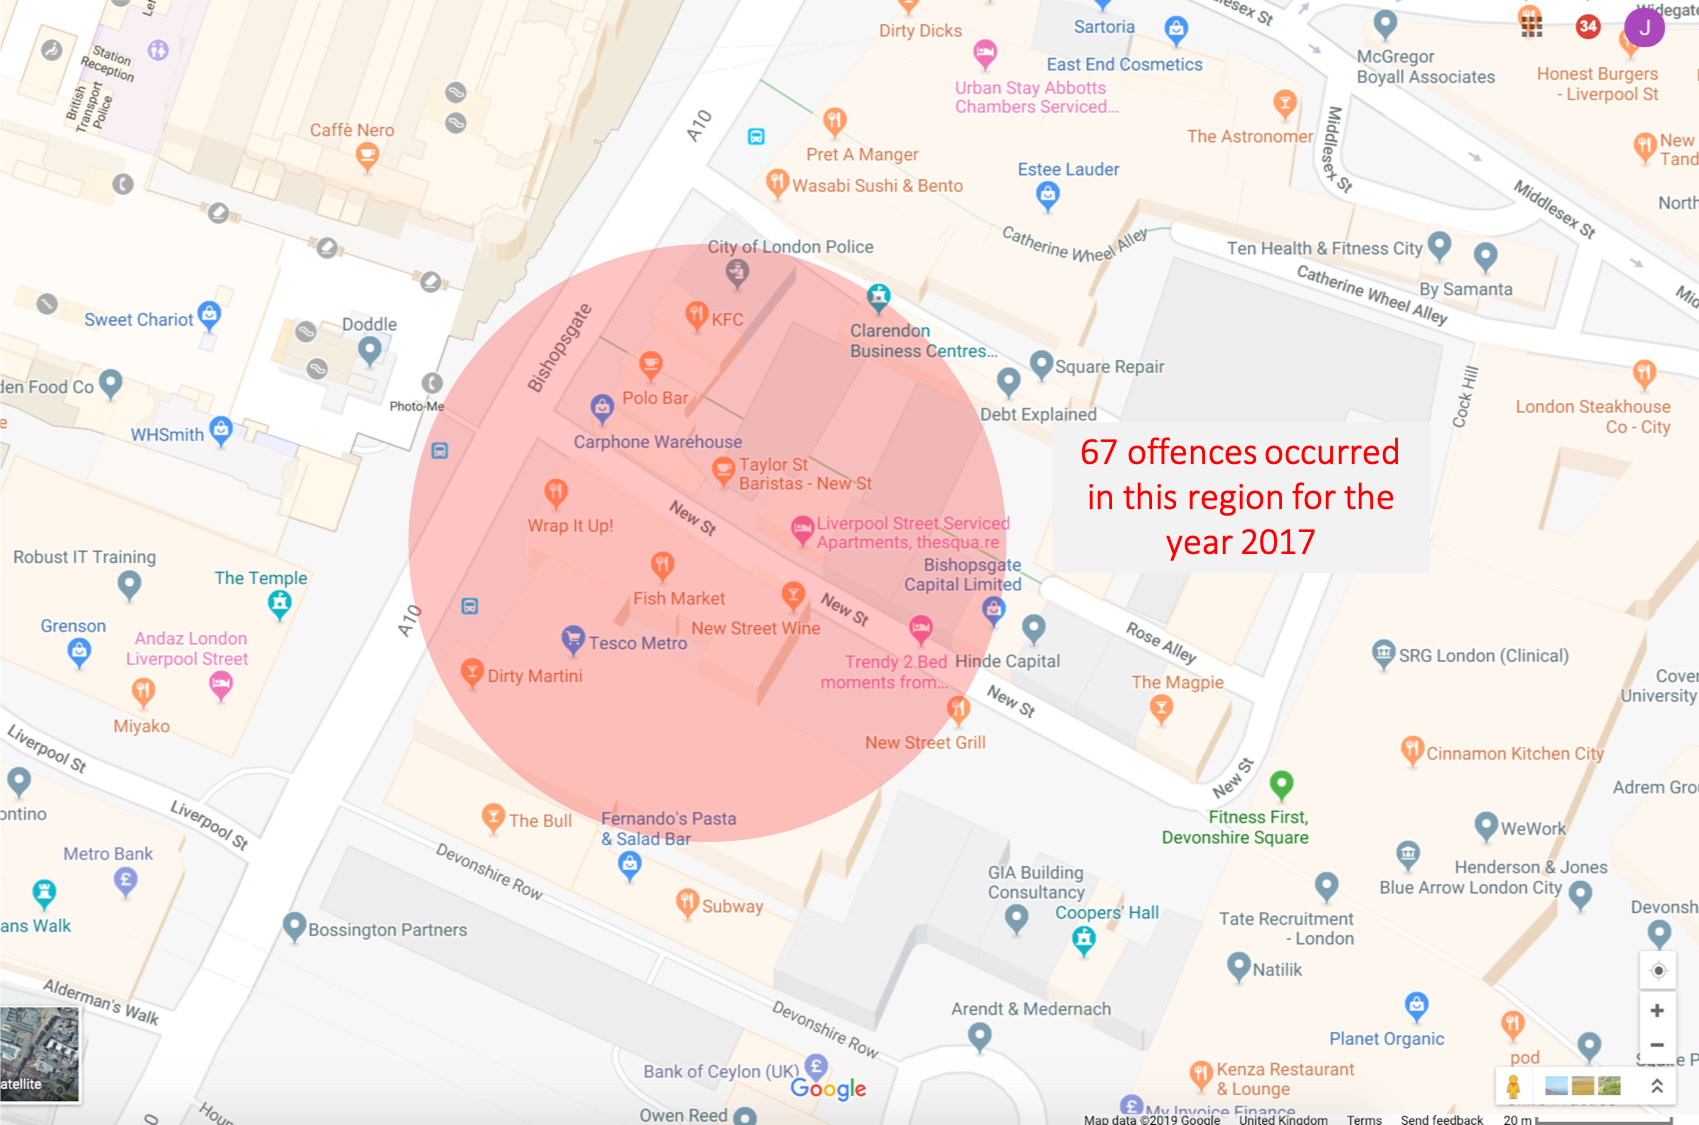
\includegraphics{pictures/COL001F_Hotspot.png}
\caption{}
\end{figure}

Based on visual inspection alone, the offences seem to congregate around
public entertainment outlets (orange markers above). Here, we construct
a second hypothesis.

H2: The location of VSO crimes correlate with the location of
entertainment outlets.

We define entertainment outlets here to be: restaurants, bars and pubs.
With open street map, we can extract the locations of these outlets and
visualise them on a map, alongside the VSO crimes:

\includegraphics{geo_project_r_files/figure-latex/COL001F-redbluedotmap-1.pdf}

Visually, the map seems to agree with our hypothesis. VSO crime
locations seem to correlate with locations of entertainment outlets. We
can perform an inhomogeneous kcross function to determine their spatial
relationship.

\includegraphics{geo_project_r_files/figure-latex/COL001F-kcross-1.pdf}

The inhomogeneous kcross function tells us that there is in fact, a
repulsive spatial relationship between the location of VSO crimes and
the location of entertainment outlets (lines below the blue line) -- VSO
crimes do not cluster around entertainment outlets.

Running a monte-carlo simulation tells us whether this observation is
statistically significant:

\begin{verbatim}
## Generating 100 simulations of CSR  ...
## 1, 2, 3, 4, 5, 6, 7, 8, 9, 10, 11, 12, 13, 14, 15, 16, 17, 18, 19, 20, 21, 22, 23, 24, 25, 26, 27, 28, 29, 30, 31, 32, 33, 34, 35, 36, 37, 38,
## 39, 40, 41, 42, 43, 44, 45, 46, 47, 48, 49, 50, 51, 52, 53, 54, 55, 56, 57, 58, 59, 60, 61, 62, 63, 64, 65, 66, 67, 68, 69, 70, 71, 72, 73, 74, 75, 76,
## 77, 78, 79, 80, 81, 82, 83, 84, 85, 86, 87, 88, 89, 90, 91, 92, 93, 94, 95, 96, 97, 98, 99,  100.
## 
## Done.
\end{verbatim}

\includegraphics{geo_project_r_files/figure-latex/COL001F-kcross-monte-1.pdf}

The observed \emph{Kcrossinhom} line lies below and outside of the
acceptance region. This means that the null hypothesis that the 2
variables are independent is rejected. The results also indicate a
dispersive relationship between the 2 variables.

This finding is surprising because we expected the 2 variables to be
attractive. We may be able to explain this finding though, that the
inhomogeneous Kcross function accounted for the the inhomogeneity in the
spatial point pattern, brought about by private buildings and parks
(random empty spaces on the map).

So although the 2 variables seem to be occurring in the `same place',
they are in fact brought together because of the spatial structure of
the environment. The presence of parks and buildings `forces' the points
to go along in a particular direction. This means if we plot other
variables on the map as well (for example: other crimes or locations of
supermarkets, etc.), their spatial locations may appear similar too --
avoiding the spaces that can't be occupied (parks, private spaces and
buildings) and occupying the spaces that can be.\\
Just out of curiosity, we can do simple tabulation of the number of VSO
crimes that happen on the streets.

\begin{table}

\caption{\label{tab:COL001F-roads-intersect}Points on the streets}
\centering
\begin{tabular}[t]{l|r}
\hline
points\_on\_roads & Freq\\
\hline
FALSE & 247\\
\hline
TRUE & 371\\
\hline
\end{tabular}
\end{table}

The results show that \textbf{60\%} of VSO crimes happen on the streets.
This may support our hypothesis that the spatial pattern of the VSO
crimes is heavily influenced by the spatial structure of the
environment.

The repulsive relationship between VSO crimes and entertainment outlets
(bars, pubs and restaurants) is still surprising though and we are
uncertain why this is so. Perhaps these are places people usually go to
with a group of friends of family and hence it is more difficult for
perpatrators to commit VSOs? These are also places with high visibility
therefore perpatrators do not dare to commit VSOs? VSOs at bars and pubs
are also likely to go unreported, because of the nature of their
environments? Or perhaps it could be because of a related variable that
causes this repulsive relationship? Clearly, more analysis and research
is needed in this area.

\hypertarget{htmlwidget-0c1675809333a60c367a}{}

\subsection{Analysing Vehicle Crime}\label{analysing-vehicle-crime}

Figure \ref{fig:vhcrimecountmap} and Figure \ref{fig:vhcrimeratemap}
show the spatial distribution of vehicle crime counts and vehicle crime
rates by LSOA respectively. Under normal circumstances, if the
relatively high crime counts are due to a large resident population, the
crime rates in these LSOAs should be relatively lower after accounting
for the size of the resident population.

However, the spatial pattern between the two maps is generally similar.
Thus, regions with the highest vehicle crime counts have the highest
vehicle crime rates, and vice versa. This can be due to two
possibilites:\\
1) Vehicle crime count is inversely proportional to resident population
size. If this is true, LSOAs with relatively high crime counts have a
small resident population, thus crime rates are also relatively high. On
the other hand, LSOAs with relatively low crime counts have a large
resident population, thus crime rates are also relatively low.\\
2) The size of the resident population in each LSOA does not have a
significant effect on the likelihood of the occurrence of vehicle crime.

Further analysis of the spatial patterns in the occurrence of vehicle
crime will be made using the crime rate map, as this is slightly more
accurate than using crime counts - the size of LSOAs varies, hence
taking crime counts alone will conflate results; crime rates attempt to
account for the variation in LSOA size. Several generalised observations
(Figure \ref{fig:vhcrimeratemap}) are described below:\\
1. Majority of LSOAs with the highest crime rates are located north of
the river Thames 2. LSOAs with the highest crime rates tend to be found
along the river Thames\\
3. LSOAs in (2) can be grouped into 4 main areas: East London
(e.g.~Newham, Barking, Greenwich), Central London (e.g.~City of London,
Westminster), Southwest London (e.g.~Kensington, Knightsbridge), West
London (e.g.~Heathrow, Acton, Hammersmith, Chiswick)

\begin{figure}
\centering
\includegraphics{geo_project_r_files/figure-latex/vhcrimecountmap-1.pdf}
\caption{\label{fig:vhcrimecountmap}2017 London vehicle crime counts by
LSOA}
\end{figure}

\begin{figure}
\centering
\includegraphics{geo_project_r_files/figure-latex/vhcrimeratemap-1.pdf}
\caption{\label{fig:vhcrimeratemap}2017 London vehicle crime rate map by
LSOA}
\end{figure}

\subsubsection{Spatial autocorrelation of vehicle
crime}\label{spatial-autocorrelation-of-vehicle-crime}

Earlier observations suggests that LSOAs with high vehicle crime rates
occur in regions. Thus, this section will investigate this further, by
examining spatial autocorrelation of vehicle crime at the LSOA level
based on regions with contiguous boundaries.

A Moran's I value of 0.36013 suggests that a positive autocorrelation in
vehicle crime counts exist on average across the entire area. Results
for the Moran's I test using randomisation and the Monte-Carlo
simulation using 999 simulations both produce small p-values of 2.2e-16
and 0.001 respectively, suggesting that the calculated Moran's I value
is highly statistically significant. Thus, at the LSOA level, frequency
of vehicle crimes display, on average, a significant positive
autocorrelation in London.

\textbf{Local spatial autocorrelation}

Local variations in spatial autocorrelation are also examined, to
determine if levels of autocorrelation vary due to spatial
heterogeneity. A map of the local Moran's I values at each LSOA is
presented in Figure \ref{fig:vhlocalmoran}.

\begin{figure}
\centering
\includegraphics{geo_project_r_files/figure-latex/vhlocalmoran-1.pdf}
\caption{\label{fig:vhlocalmoran}2017 London vehicle crime rates local
Moran's by LSOA}
\end{figure}

LSOAs with local Moran's I values that are statistically significant at
the 95\% confidence interval were then calculated and mapped. Figure
\ref{fig:vhmorancluster} shows that spatial autocorrelation is
non-significant across most of London. It is however noteworthy that the
LSOAs with the highest crime rates also tend to form statistically
significant high-high clusters. Specifically, high-high clusters are
present in West London, central London and East London along the river
Thames. This confirms the earlier hypothesis that there is a
concentration of crimes on a local level in different regions of London.
It is also notable that several other LSOAs (that do not have relatively
high vehicle crime rates) also have high-high clusters, indicating that
spatial autocorrelation is not only restricted to regions with high
vehicle crime rates. This may be related to characteristics of the
region or criminal behaviour. Interestingly, a single low-low cluster is
observed in south London, in the Bexley region.

\begin{figure}
\centering
\includegraphics{geo_project_r_files/figure-latex/vhmorancluster-1.pdf}
\caption{\label{fig:vhmorancluster}LSOAs with statistically significant
local Moran's clusters for vehicle crime}
\end{figure}

\subsubsection{Reasons for vehicle crime
rates}\label{reasons-for-vehicle-crime-rates}

Earlier analysis reveals that elevated crime rates tend to occur in
specific regions, and there is spatial autocorrelation at the LSOA
level. Therefore, this section will examine regions with high vehicle
crime rates to identify variables that may contribute to high crime
rates.

\textbf{East London}

In East London, the LSOAs with high crime rates either have 1)
industrial parks/scrapyards/depots (e.g.~Barking LSOAs, Newham LSOAs)
and/or 2) retail parks/leisure parks (e.g.~Newham LSOAs, Greenwich
LSOAs). For instance, the agglomeration of retail parks in Newham (and
the accompanying parking lots), such as the Gallions reach shopping
park, Beckton Triangle retail park and Gateway retail park may
contribute to the elevated vehicle crime rates in the LSOA. Likewise, in
Greenwich, the presence of leisure parks and the O2 stadium may
contribute to the high vehicle crime rates. The high vehicle crime rates
at retail parks/leisure parks suggests that thieves are likely
opportunistic, and target these areas due to the high volume of vehicles
parked in these areas.

On the other hand, in parts of Creekmouth and Barking, the high vehicle
crime rates may be attributed to industrial parks and scrapyards. The
high rates of vehicle crime at industrial areas is interesting, as the
vehicles are often old and/or damaged. This suggests that thieves may
steal vehicle parts from these areas. Industrial areas are also
relatively quiet and empty at night, which may mean that the risk of
getting caught is lower. The perceived risk may be a contributory factor
to the higher crime rates.

\begin{figure}
\centering
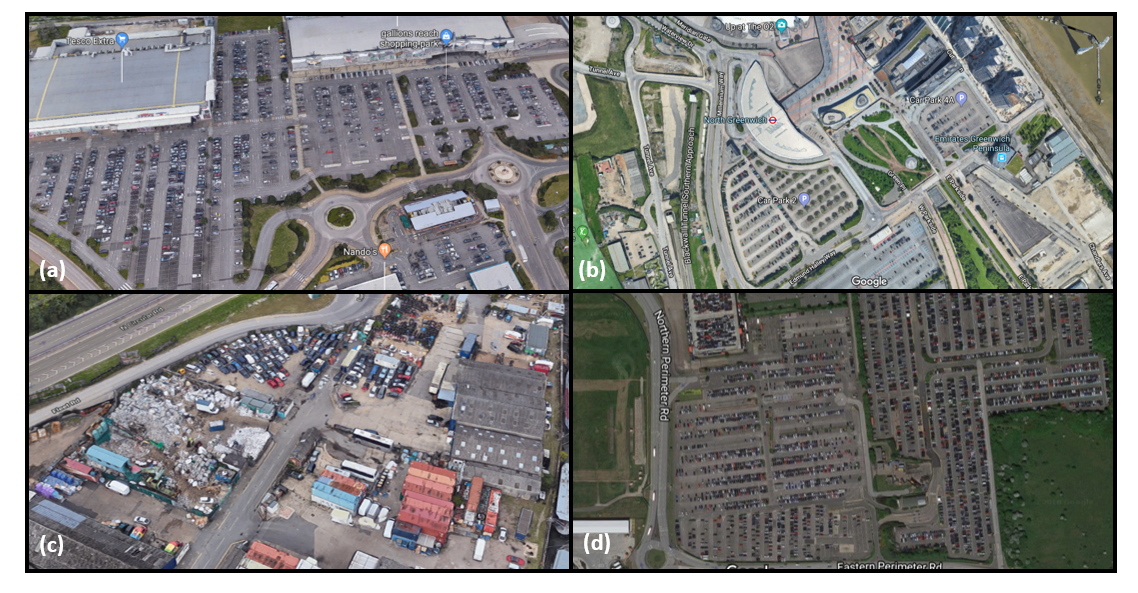
\includegraphics{pictures/parkedcars.png}
\caption{Parked vehicles (a) Parking lots at retail parks at Newham, (b)
Parking lots at the O2 stadium and leisure park in Greenwich, (c)
Vehicles at industrial area in Barking, (d) Parked vehicles at Heathrow
airport}
\end{figure}

\textbf{West London}

Interestingly, crime patterns are different in West London and can
generally be linked to either carparks or car dealers. High rates of
vehicle crime near Heathrow airport may be attributed to the high
volumes of parked vehicles at short-stay and long-stay carparks.
Criminals may therefore choose to operate near the airport, particularly
at the long-stay carparks which are likely used by individuals
travelling abroad.

The high crime rates in Chiswick may also be linked to the presence of
large numbers of parked cars, as the LSOAs with the highest crime rates
tend to have either carparks associated with supermarkets or car
dealers. These observations are consistent with the hypothesis that
thieves are opportunistic, and pick areas with more parked vehicles.

However, these hypotheses do not apply to Hammersmith and parts of
Hounslow, both of which appear to be predominantly residential. It may
be possible that these LSOAs have high crime rates as they are in the
vicinity of other hotspots, such as those in Chiswick.

Vehicle crime rates are also high in Richmond, and may be linked to the
presence of multiple carparks and the affluent demographic of the area.

\textbf{Southwest London}

In contrast to other regions, where high crime rates are associated with
industrial and commercial areas, in Southwest London, high vehicle crime
rates occur in residential areas such as Kensington, Chelsea and
Knightsbridge. Unlike other areas, the volume of parked vehicles is not
exceptionally high - there are no carparks/industrial areas/car dealers.
However, there are numerous luxury vehicles parked in these areas, as
they are affluent neighbourhoods. Hence, it is likely that vehicle crime
rates are high in these region, as thieves operating in these areas
specifically target high-value vehicles.

\begin{figure}
\centering
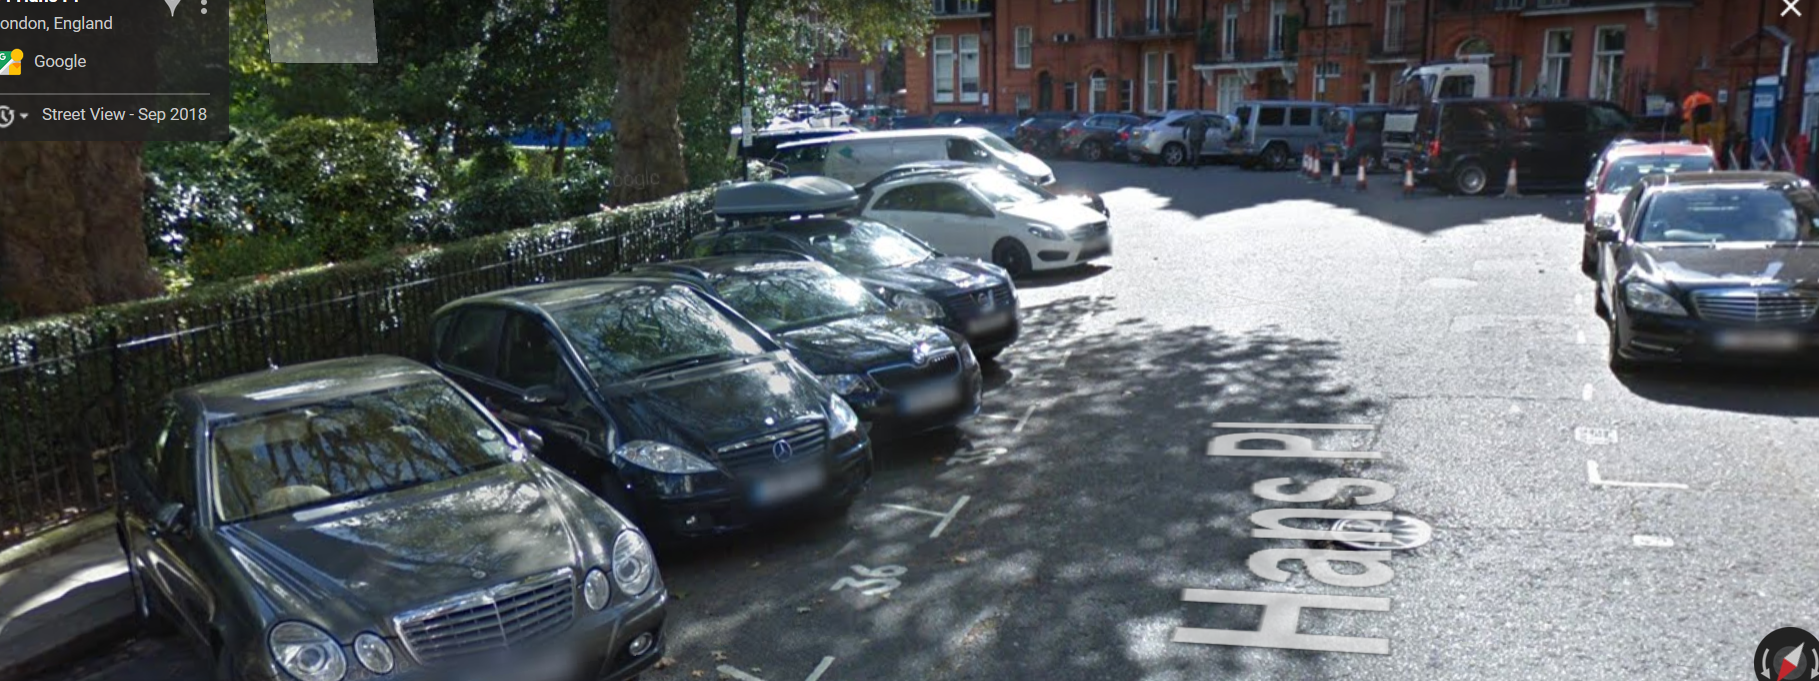
\includegraphics{pictures/Knightsbridge.png}
\caption{Luxury vehicles in Knightsbridge}
\end{figure}

\textbf{Central London}

It is not clear why vehicle crime rates are high in central London,
particularly in the City of London and Westminster. However, it is also
interesting that some parts of the City of London (e.g.~Moorgate,
Barbican) have low vehicle crime rates - this may be due to the presence
of secure parking in underground carparks.

\subsubsection{Discussion}\label{discussion}

More detailed examination of regions with high vehicle crime rates
suggests two main modes of operation for criminals:\\
1) Operating in areas with large numbers of parked vehicles
(i.e.~quantity over quality{]} ) 2) Operating specifically in affluent
areas to target high-value vehicles (i.e.~quality over quantity)

Based on hypothesis (1), further analysis has identified industrial
areas and large carparks to be significant variables associated with
elevated vehicle crime rates. A map of industrial areas and the vehicle
crime rates by LSOAs is therefore generated to visualise the
relationship between vehicle crime rates and industrial areas (Figure
\ref{fig:industrialmap}). There appears to be a correlation between
industrial areas and vehicle crime rates. This may be because these
areas tend to be quiet at night thus, the risk of getting caught is
lower. Future work to model vehicle crime patterns can therefore
consider including distance from industrial areas as one of the
variables to be modelled. Distances to the nearest police station can
also be considered as a proxy for perceived risk of getting caught.

Ideally, the relationship between large carparks (as a proxy for the
number of parked vehicles) and vehicle crime rates will also be
visualised. However, datasets for carparks are not fully complete - for
instance, the data on OpenStreetMap mainly limited to central London.
Moreover, the dataset provides information on general parking spaces
(which could be anywhere), and not the location of large carparks.
Future work can consider examining the relationship between large car
parks and vehicle crime rates.

Based on hypothesis (2), future work can consider incorporating income
data in residential areas as a variable contributing to vehicle crime
rates.

That said, high crime rates in central London and other residential (but
not particularly affluent) parts of West London such as Hammersmith
cannot be explained using the above hypotheses. Further studies can look
towards understanding criminal behaviour in these regions.

Lastly, analysis of the vehicle crime dataset is conducted in the form
of areal analysis at the LSOAs level. Different levels of analysis may
produce different results, and a higher level of aggregation (e.g.~at
the borough level) may produce different trends. Whilst the observations
at the broader areal level between LSOAs suggests that a relationship
between industrial areas, car parks with vehicle crime, as well as a
relationship between affluent areas and high-value vehicle crime exists,
more detailed point analyses at a local level may suggest otherwise.
Thus, further work can be conducted within LSOAs, to examine the
interactions between these variables at a local level.

\begin{figure}
\centering
\includegraphics{geo_project_r_files/figure-latex/industrialmap-1.pdf}
\caption{\label{fig:industrialmap}Location of carparks and industrial areas
on top of vehicle crime rates}
\end{figure}

\pagebreak

\section{Conclusion}\label{conclusion}

In conclusion, visual analysis of the location of entertainment outlets
and VSO crimes suggest that they are positively correlated. However,
further statistical analysis indicates that a repulsive relationship
exists between the two. This scenario underpins the importance of
rigorous statistical analysis in testing observations. The reasons for
the repulsive relationship are unknown, and further research can be
conducted in this area. This can include the incorporation of pedestrian
footfall data.

Areal analysis of vehicle crime rates at the LSOAs level indicates
cluters of high vehicle crime in parts of West London, East London,
Central London and Southwest London. Several hypotheses for these
cluster have been formulated. Specifically, these clusters may be
attributed to 1) large numbers of parked vehicles, or 2) a concentration
of high-end vehicles. Future work can looking into quantifying the
effect of variables such as the distance from industrial areas,
carparks, and the nearest police station. Analysis at the LSOA level is
subject to the modifiable areal unit problem, and further investigation
of the individual points can be considered to better understand the
dynamics at the local level. The limitations of a localised point-based
analysis can thus be partially addressed using a broader areal-level
analysis, and vice versa.

As such, an integrated approach will be the best approach.

\pagebreak

\section{References}\label{references}

\hypertarget{refs}{}
\hypertarget{ref-Anselin1995}{}
Anselin, Luc. 1995. ``Local indicators of spatial analysis--LISA.''
\emph{Geographical Analysis} 27 (2): 93--115.
doi:\href{https://doi.org/10.1111/j.1538-4632.1995.tb00338.x}{10.1111/j.1538-4632.1995.tb00338.x}.

\hypertarget{ref-Basiri2016}{}
Basiri, Anahid, Mike Jackson, Pouria Amirian, Amir Pourabdollah, Monika
Sester, Adam Winstanley, Terry Moore, and Lijuan Zhang. 2016. ``Quality
assessment of OpenStreetMap data using trajectory mining.''
\emph{Geo-Spatial Information Science} 19 (1). Taylor \& Francis:
56--68.
doi:\href{https://doi.org/10.1080/10095020.2016.1151213}{10.1080/10095020.2016.1151213}.

\hypertarget{ref-Brand2014}{}
Brand, Sam, and Richard Price. 2014. ``The Economic and Social Costs of
Crime.'' \emph{Home Office Research Study 217}, no. July.

\hypertarget{ref-Brantingham1997}{}
Brantingham, P L, and P J Brantingham. 1997. ``Mapping Crime for
Analytic Purposes: Location Quotients, Counts and Rates.'' \emph{Mapping
Crime for Analytic Purposes: Location Quotients, Counts and Rates}, no.
May: 263--88.
doi:\href{https://doi.org/10.1016/j.amc.2008.06.050}{10.1016/j.amc.2008.06.050}.

\hypertarget{ref-Chainey2008}{}
Chainey, Spencer, Lisa Tompson, and Sebastian Uhlig. 2008. ``The Utility
of Hotspot Mapping for Predicting Spatial Patterns of Crime.''
\emph{Security Journal} 21 (4): 291--92.
doi:\href{https://doi.org/10.1057/sj.2008.6}{10.1057/sj.2008.6}.

\hypertarget{ref-Cheng2012}{}
Cheng, T, and D Williams. 2012. ``Space-time analysis of crime patterns
in central London.'' \emph{International Archives of the Photogrammetry,
Remote Sensing and Spatial Information Sciences - ISPRS Archives} 39
(September): 47--52.
doi:\href{https://doi.org/10.5194/isprsarchives-XXXIX-B2-47-2012}{10.5194/isprsarchives-XXXIX-B2-47-2012}.

\hypertarget{ref-Office2019}{}
Home Office. 2019. ``About data.police.uk.''
\url{https://data.police.uk/about/}.

\hypertarget{ref-Malleson2016}{}
Malleson, Nick, and Martin A. Andresen. 2016. ``Exploring the impact of
ambient population measures on London crime hotspots.'' \emph{Journal of
Criminal Justice} 46. The Authors: 52--63.
doi:\href{https://doi.org/10.1016/j.jcrimjus.2016.03.002}{10.1016/j.jcrimjus.2016.03.002}.

\hypertarget{ref-MayorofLondon2016}{}
Mayor of London. 2016. ``A City for all Londoners,'' 1--84.
\href{https://www.london.gov.uk/sites/default/files/city\%7B/_\%7Dfor\%7B/_\%7Dall\%7B/_\%7Dlondoners\%7B/_\%7Dnov\%7B/_\%7D2016.pdf}{https://www.london.gov.uk/sites/default/files/city\{\textbackslash{}\_\}for\{\textbackslash{}\_\}all\{\textbackslash{}\_\}londoners\{\textbackslash{}\_\}nov\{\textbackslash{}\_\}2016.pdf}.

\hypertarget{ref-Moran1950}{}
Moran, P A P. 1950. ``Notes on continuous stochastic processes.''
\emph{Biometrika} 37 (3): 17--23.

\hypertarget{ref-Sherman1989}{}
Sherman, Lawrence W., Patrick R. Gartin, and Michael E. Buerger. 1989.
``Hot spots of predatory crime: Routine activities and the criminology
of place.'' \emph{Criminology} 27 (1): 27--56.
doi:\href{https://doi.org/10.1111/j.1745-9125.1989.tb00862.x}{10.1111/j.1745-9125.1989.tb00862.x}.

\hypertarget{ref-Tompson2015}{}
Tompson, Lisa, Shane Johnson, Matthew Ashby, Chloe Perkins, and Phillip
Edwards. 2015. ``UK open source crime data: Accuracy and possibilities
for research.'' \emph{Cartography and Geographic Information Science} 42
(2). Taylor \& Francis: 97--111.
doi:\href{https://doi.org/10.1080/15230406.2014.972456}{10.1080/15230406.2014.972456}.


\end{document}
